\documentclass{beamer}
\mode<presentation>
\usetheme{CambridgeUS}
\usepackage[russian]{babel}
\usepackage[utf8]{inputenc}
\usepackage[T2A]{fontenc}
\usepackage{sansmathaccent}

\usepackage{verbatim}
\usepackage{alltt}

\pdfmapfile{+sansmathaccent.map}
\title[Шаблоны]{Шаблоны}
\author{Наумов Д.А., доц. каф. КТ}
\date[21.10.2020] {Компьютерная графика и проектирование графических интерфейсов, 2020}

\begin{document}

%ТИТУЛЬНЫЙ СЛАЙД
\begin{frame}
  \titlepage
\end{frame}
  
%СОДЕРЖАНИЕ ЛЕКЦИИ
\begin{frame}
  \frametitle{Содержание лекции}
  \tableofcontents  
\end{frame}

\section{Шаблоны}

\subsection{Общая информация о шаблонах}

\begin{frame}[t]
	Тенденции, связанные с UI/UX design:
	\begin{itemize}
		\item быстрое распространие интерфейсов-идиом (легко узнаваемые типы интерфейсов с собственным запаос объектов, действий и визуальных элементов);
		\item ослабление правил сборки интерфейсов на базе идиом (смешение стилей).
		\begin{itemize}
			\item фрагменты текстовой справки + формы и редакторы;
			\item формы выбора с использованием броских макетов (списки, календари).			
		\end{itemize}
	\end{itemize}
	\begin{figure}[h]
		\centering
		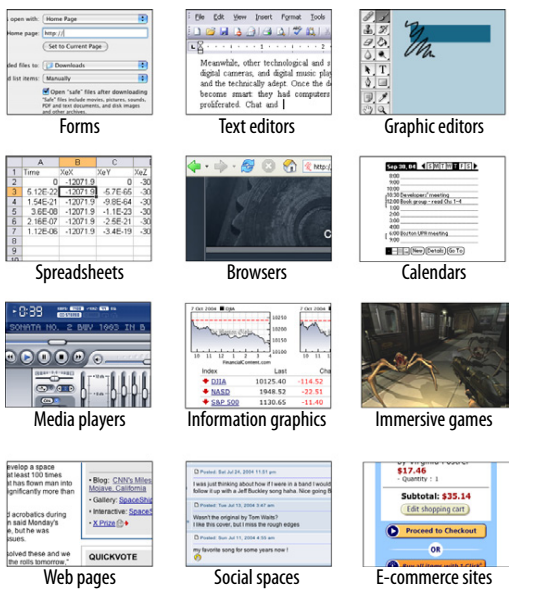
\includegraphics[scale=0.5]{images/lec06-pic01.png}
	\end{figure}
\end{frame} 

\begin{frame}[t]
	\begin{block}{Шаблон}
		стурктурные и поведенческие характеристики, улучшающие пригодность чего-либо: пользовательского интерфейса, веб-сайта, объектно-ориентированной программы.
	\end{block}
	Шаблоны - описание рекомендуемых практик в области дизайна.
	\begin{itemize}
		\item фиксируют распространенные ответы на сложные вопросы;
		\item не являются готовыми к применению компонентами (каждая реализация шаблона будет отличаться от остальных);
		\item не смогут служить гидом в последовательности решений по созданию дизайна;
		\item независимы от платформы или системы;
		\item определяют некоторые возможности, а не ограничения;
		\item представляют собой связь между многими элементами, а не единственный элемент;
		\item настраиваются в зависимости от контекста.
	\end{itemize}	
\end{frame} 

\subsection{Поведеческие шаблоны}

\begin{frame}[t]	
	\begin{block}{Поведеческие шаблоны}
		описывают человеческое поведение, а не элементы интерфейса.
	\end{block}
	\textit{Люди уникальны, но их поведение довольно предсказуемо.}
	\begin{enumerate}
		\item Safe Exploration - безопасное исследование;
		\item Instant Gratification - мгновенное вознаграждение;
		\item Satisficing - разумная достаточность;
		\item Changes in Midstream - изменения на полпути;
		\item Deferred Choices - отложенный выбор;
		\item Incremental Construction - пошаговое построение;
		\item Habituation - привыкание;
		\item Spatial Memory - пространственная память;
		\item Prospective Memory - проспективная память;
		\item Streamlined Repetition - организационное построение;
		\item Keyboard Only - только клавиатура;
		\item Other People’s Advice - советы других людей.
	\end{enumerate}	
\end{frame} 

\begin{frame}[t]	
	\begin{block}{Safe Exploration (безопасное исследование)}
		 позвольте мне исследовать программу, не теряясь в ней и не попадая в неприятности.		 
	\end{block}
	<<Неприятности>>
	\begin{itemize}
		\item закрытие всплывающих окон;
		\item повторный ввод ошибочно стертых данных;
		\item поспешное отключение звука.				
	\end{itemize}
	\textbf{Пример}: 
	\begin{itemize}
		\item сохранение документа,
		\item редактирование фотографий, 
		\item исследование сайта.				
	\end{itemize}	
\end{frame}

\begin{frame}[t]	
	\begin{block}{Instant Gratification (мгновенное вознаграждение)}
		 я хочу видеть результат действий прямо сейчас!
	\end{block}
	\begin{itemize}
		\item графический редактор: холст, палитра, выбранный инструмент рисования;
		\item решение задачи: начать с типичной отправной точки.
	\end{itemize}
	Не следует прятать начальную функциональность:
	\begin{itemize}
		\item за тем, что должно быть прочитано;
		\item за тем, чего нужно долго ждать.	
	\end{itemize}	
\end{frame}

\begin{frame}[t]	
	\begin{block}{Satisficing (разумная достаточность)}
		 меня это устраивает, я не хочу тратить время на то, чтобы выучить что-то еще или как сделать это лучше.
	\end{block}	
	Satisficing = satisfying + sufficing (удовлетворительный + достаточный)
	~
	Herbert Simon, 1957: \textit{люди предпочитают довольствоваться достаточно хорошим, а не наилучшим, если изучение всех альтернативных вариантов может требовать траты лишнего времени и усилий.}
	\begin{itemize}
		\item предусмотреть несколько варинатов действий;
		\item высока вероятность, что пользователь попробует один из них;
		\item если выбор будет неправильный, то пользователь вернется на шаг назад.		
	\end{itemize}
	Рекомендации для дизайнеров:
	\begin{itemize}
		\item используйте короткие метки и простые слова;
		\item макет интерфейса должен отражать суть приложения;
		\item продумайте простой способ перемещения	по интерфейсу;
		\item сложный интерфейс предъявляет высокие когнитивные требования к пользователям.
	\end{itemize}	
\end{frame}

\begin{frame}[t]	
	\begin{block}{Changes in Midstream (изменения на полпути)}
		 я передумал, пока делал что-то.
	\end{block}	
	\textit{Первоначальные цели пользователей могут измениться.}
	~
	Рекомендации для дизайнеров:
	\begin{itemize}
		\item дать пользователю выбор, возможность изменить поставленную цель;
		\item не <<запирайте>> пользователя в среде с ограниченным выбором без причиин
		\begin{itemize}
			\item шаблон Wizard;
			\item шаблон Modal Panel.			
		\end{itemize}
		\item упростить запуск процесса, остановку в середине и возвращение в точку останова;
		\item используйте Good Defaults - хорошие варианты по умолчанию;		
		\item меньше использовать диалоговые окна (для редактора).		
	\end{itemize}	
\end{frame}

\begin{frame}[t]	
	\begin{block}{Deferred Choices (отложенный выбор)}
		 я не хочу отвечать на этот вопрос прямо сейчас!
	\end{block}	
	\textit{Если задать пользователю несколько незначительных вопросов, пока он пытается выполнить какую-то задачу, он, скорее всего, пропустит вопросы, чтобы вернуться к ним позже.}
	\begin{itemize}
		\item долгая регистрация на доске объявлений;
		\item создание проекта в Adobe Premiere;		
		\item нежелание отвечать на вопрос (сейчас или вообще);				
		\item отсутствие информации в данный момент.		
	\end{itemize}		
	Рекомендации для дизайнеров:
	\begin{itemize}
		\item помечайте необходимые для заполнения поля;	
		\item не приставайте к пользователю со слишком большим списком вопросов;
		\item отделяйте важные и не	важные вопросы;
		\item используйте Good Defaults - хорошие варианты по умолчанию;
		\item обеспечьте возможность вернуться в отложенным вопросам.						
	\end{itemize}	
\end{frame}

\begin{frame}[t]	
	\begin{block}{Incremental Construction (пошаговое построение)}
		 дайте мне это изменить! Нет, опять неправильно. Попробую еще раз. Вот так-то лучше.
	\end{block}	
	\textit{Когда пользователи создают что-то, они обычно не завершают работу за один раз.}
	Рекомендации для дизайнеров:
	\begin{itemize}
		\item предусмотрите возможность создания небольших фрагментов;
		\item сделайте интерфейс восприимчивым к быстрым изменениями и частым сохранениями;		
		\item демонстрируйте, как будет выглядеть результат;		
		\item делайте этам компиляции максимально быстрым;		
		\item пользователь должен вовлекаться в процесс работы.		
	\end{itemize}	
\end{frame}

\begin{frame}[t]	
	\begin{block}{Habituation (привыкание)}
		 этот способ работает везде, почему же он не работает здесь?
	\end{block}	
	\textit{Когда пользователи постоянно работают в одном интерфейсе, некоторые часто изпользуемые физические действия становятся рефлекторными.}
	\begin{itemize}
		\item Ctrl+S
		\item кнопка <<Назад>>
		\item клавивша Enter в модальном окне.
	\end{itemize}
	Привыкание может скрывать за собой ловушки:		
	\begin{itemize}
		\item Ctrl+X, Ctrl+S - сохранение в emacs;
		\item Ctrl+A - перемещение к началу строки в emacs;
	\end{itemize}
	\textit{А если бы это был Microsoft Word?}
	~
	Рекомендации для дизайнеров:
	\begin{itemize}
		\item единообразие в рамках одного приложения;
		\item единообразие в рамках привычных пользователю приложений.
	\end{itemize}	
\end{frame}

\begin{frame}[t]	
	\begin{block}{Spatial Memory (пространственная память)}
		 клянусь, эта кнопка была здесь! Куда она пропала?
	\end{block}	
	\textit{Когда пользователи работают с объектами и документами, то часто возвращаются к ним, ориентируясь на свои воспоминания об их местоположении, а не восстанавливая в памяти фактические пути и названия.}
	\begin{itemize}
		\item рабочий стол (варианты группирования значков);
		\item размещение кнопок Ok, Cancel в предсказуемых местах;
		\item динамическое изменение меню имеет непрятные последствия.
	\end{itemize}
	Рекомендации для дизайнеров:
	\begin{itemize}
		\item добавление элементом вызывает мешьше проблем, чем перемещение знакомых элементов;
		\item представить пользователям возможность самостоятельно упорядочивать объекты.
		\item верхние и нижние области списков и меню - особые места в когнитивном смысле: люди их лучше запоминают, их лучше не менять.		
	\end{itemize}	
\end{frame}

\begin{frame}[t]	
	\begin{block}{Prospective Memory (проспективная память)}
		 оставлю это здесь, чтобы не забыть заняться этим позже.
	\end{block}	
	\textit{Проспективная память используется, когда мы планируем сделать что-то в будущем и организуем некий способ напомнить себе о необходимости сделать это.}
	\begin{itemize}
		\item листок-напоминание;
		\item книга на столике у входной двери;
		\item настроенные звуковые сигналы таймера.
		\item примечания прямо в документе;
		\item закладки в браузере;
		\item документ на рабочем столе;		
		\item письмо в папке <<входящие>>;				
	\end{itemize}
	Рекомендации для дизайнеров:
	\begin{itemize}
		\item гибкость инструментов;
		\item невмешательство в работу пользователя.
		\item напомнинание пользователю (списки последних объектов).
	\end{itemize}	
\end{frame}

\begin{frame}[t]	
	\begin{block}{Streamlined Repetition (организационное построение)}
		 сколько раз мне нужно это повторить?!
	\end{block}	
	\textit{Пользователям иногда приходится выполнять одну и ту же операцию снова и снова; задача - упростить пользователям это действие.}
	\begin{itemize}
		\item Find and Replace - Replace All
		\item макросы и сценарии;		
		\item простое повторение команд;
		\item исползование копирования и вставки;		
	\end{itemize}
	Рекомендации для дизайнеров:
	\begin{itemize}
		\item изучать действия пользователей;
		\item предложить пользователям способ упрощения повторяющихся задач.
	\end{itemize}	
\end{frame}

\begin{frame}[t]	
	\begin{block}{Keyboard Only (только клавиатура)}
		 пожалуйста, не заставляйте меня использовать мышь.
	\end{block}	
	\textit{Пользователям предпочитают не переключаться между мышью и клавиатурой; лучше они постоянно будут держат руки на клавиатуре.}
	\begin{itemize}
		\item нет операций, которые можно выполнить только мышью (для приложений, работающих с данными);
		\item определить сочетания клавишь;
		\item быстрый доступ в меню (Alt);
		\item выбор нескольких вариантов (Shift, Ctrl);		
		\item перемещение - Tab, Shift-Tab;
		\item перемещение - вообще без Tab;		
		\item выбор при помощи стрелок и клавиши <<пробел>>;
		\item операция по-умолчанию - Enter.				
	\end{itemize}
\end{frame}

\begin{frame}[t]	
	\begin{block}{Other People’s Advice (советы других людей)}
		 а что другие люди говорят об этом?
	\end{block}	
	\textit{Люди - социальные существа. На наше собственное мнение влияет то, что говорят коллеги.}
	\begin{itemize}
		\item возможность комментирования в интерактивном режиме;
		\item отызвы на продукты, товары, услуги;
		\item how-to;
		\item публичная оценка.		
	\end{itemize}
	Рекомендации для дизайнеров:
	\begin{itemize}
		\item не может ли повысить эффективность работы пользователей введение социального компонента;
		\item шаблон Multi-level Help.
	\end{itemize}		
\end{frame}

\end{document}
